
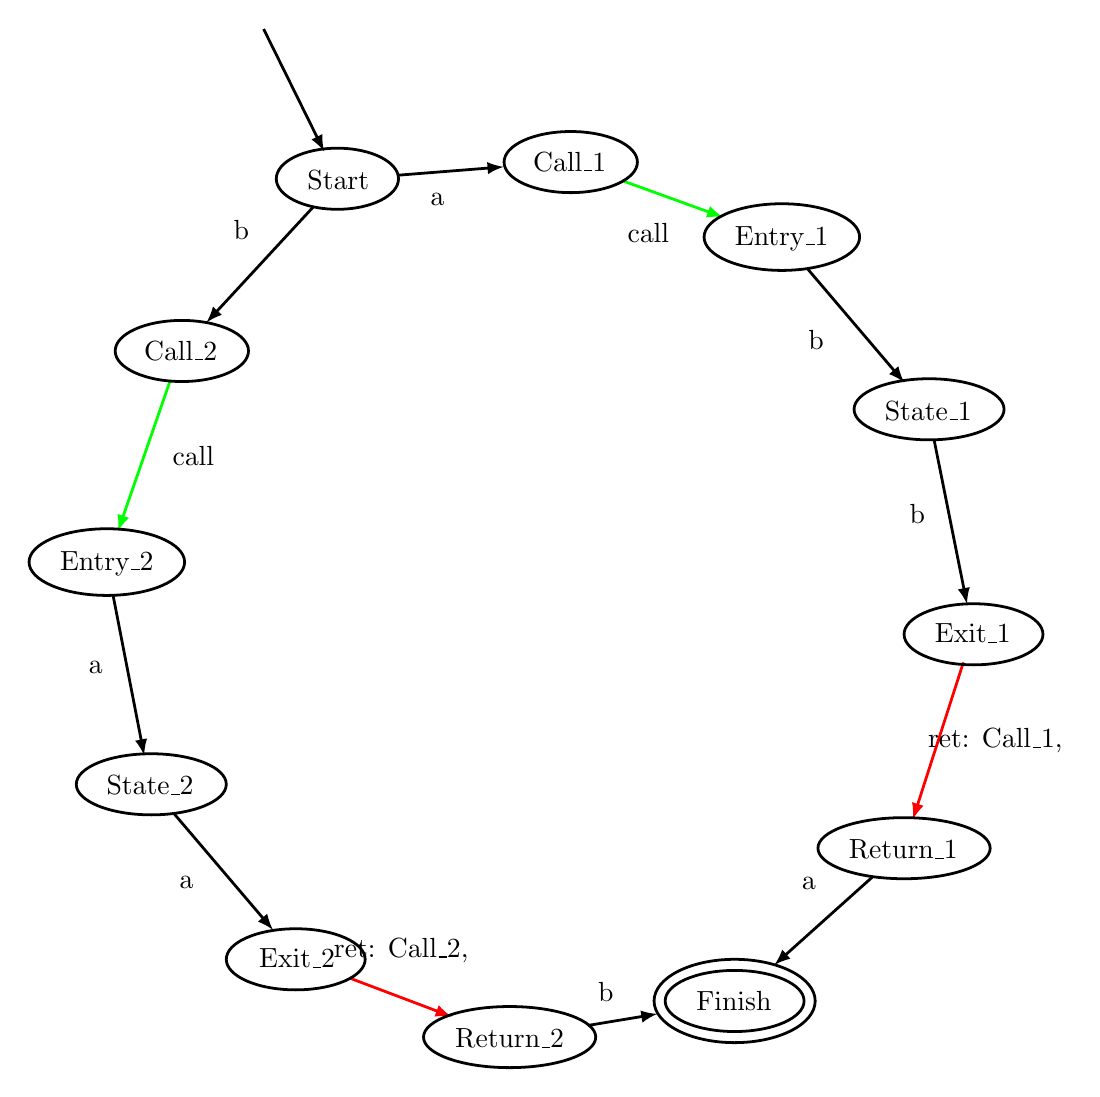
\begin{tikzpicture}[>=latex,line join=bevel,]
  \pgfsetlinewidth{1bp}
%%
\pgfsetcolor{black}
  % Edge: Return_1 -> Finish
  \draw [->] (304.51bp,69.534bp) .. controls (296.77bp,62.602bp) and (286.22bp,53.146bp)  .. (269.29bp,37.968bp);
  \definecolor{strokecol}{rgb}{0.0,0.0,0.0};
  \pgfsetstrokecolor{strokecol}
  \draw (281.66bp,67.128bp) node {a};
  % Edge: Exit_2 -> Return_2
  \pgfsetcolor{red}
  \draw [->] (116.4bp,33.253bp) .. controls (124.58bp,30.16bp) and (134.38bp,26.461bp)  .. (153.14bp,19.373bp);
  \definecolor{strokecol}{rgb}{0.0,0.0,0.0};
  \pgfsetstrokecolor{strokecol}
  \draw (134.97bp,43.126bp) node {ret: Call\_2, };
  % Edge: Call_1 -> Entry_1
  \pgfsetcolor{green}
  \draw [->] (214.5bp,320.33bp) .. controls (222.6bp,317.39bp) and (232.28bp,313.89bp)  .. (250.87bp,307.15bp);
  \definecolor{strokecol}{rgb}{0.0,0.0,0.0};
  \pgfsetstrokecolor{strokecol}
  \draw (223.93bp,301.46bp) node {call};
  % Edge: State_2 -> Exit_2
  \draw [->] (53.049bp,92.599bp) .. controls (60.876bp,83.405bp) and (72.669bp,69.55bp)  .. (88.826bp,50.571bp);
  \draw (57.595bp,67.512bp) node {a};
  % Edge: State_1 -> Exit_1
  \draw [->] (326.8bp,227.04bp) .. controls (329.3bp,214.56bp) and (333.53bp,193.44bp)  .. (338.65bp,167.88bp);
  \draw (320.74bp,200.38bp) node {b};
  % Edge: Return_2 -> Finish
  \draw [->] (202.22bp,16.192bp) .. controls (207.03bp,16.99bp) and (212.09bp,17.831bp)  .. (227.18bp,20.339bp);
  \draw (208.65bp,28.427bp) node {b};
  % Edge: Start -> Call_2
  \draw [->] (103.19bp,310.71bp) .. controls (94.718bp,301.55bp) and (81.916bp,287.69bp)  .. (64.853bp,269.23bp);
  \draw (77.453bp,302.68bp) node {b};
  % Edge: Call_2 -> Entry_2
  \pgfsetcolor{green}
  \draw [->] (51.878bp,248.54bp) .. controls (47.884bp,237.02bp) and (41.416bp,218.37bp)  .. (33.011bp,194.14bp);
  \definecolor{strokecol}{rgb}{0.0,0.0,0.0};
  \pgfsetstrokecolor{strokecol}
  \draw (60.126bp,221.19bp) node {call};
  % Edge: Start -> Call_1
  \draw [->] (134.2bp,322.3bp) .. controls (142.61bp,322.97bp) and (152.42bp,323.74bp)  .. (171.84bp,325.28bp);
  \draw (147.95bp,313.39bp) node {a};
  % Edge: Exit_1 -> Return_1
  \pgfsetcolor{red}
  \draw [->] (337.36bp,146.91bp) .. controls (333.54bp,135.02bp) and (327.21bp,115.35bp)  .. (319.17bp,90.389bp);
  \definecolor{strokecol}{rgb}{0.0,0.0,0.0};
  \pgfsetstrokecolor{strokecol}
  \draw (348.87bp,118.62bp) node {ret: Call\_1, };
  % Edge: Entry_1 -> State_1
  \draw [->] (281.37bp,288.43bp) .. controls (289.13bp,279.31bp) and (300.3bp,266.19bp)  .. (316.05bp,247.68bp);
  \draw (284.36bp,262.99bp) node {b};
  % Edge: Entry_2 -> State_2
  \draw [->] (31.293bp,170.77bp) .. controls (33.713bp,158.32bp) and (37.572bp,138.46bp)  .. (42.44bp,113.41bp);
  \draw (24.898bp,145.08bp) node {a};
  % Edge: Start__precursor__ -> Start
  \draw [->] (85.447bp,374.89bp) .. controls (90.652bp,364.36bp) and (97.308bp,350.9bp)  .. (107.2bp,330.89bp);
  % Node: Finish
\begin{scope}
  \definecolor{strokecol}{rgb}{0.0,0.0,0.0};
  \pgfsetstrokecolor{strokecol}
  \draw (255bp,25bp) ellipse (25bp and 11bp);
  \draw (255bp,25bp) ellipse (29bp and 15bp);
  \draw (254.72bp,24.915bp) node {Finish};
\end{scope}
  % Node: Return_2
\begin{scope}
  \definecolor{strokecol}{rgb}{0.0,0.0,0.0};
  \pgfsetstrokecolor{strokecol}
  \draw (174bp,12bp) ellipse (31bp and 11bp);
  \draw (173.98bp,11.5bp) node {Return\_2};
\end{scope}
  % Node: Start
\begin{scope}
  \definecolor{strokecol}{rgb}{0.0,0.0,0.0};
  \pgfsetstrokecolor{strokecol}
  \draw (112bp,321bp) ellipse (22bp and 11bp);
  \draw (112.3bp,320.57bp) node {Start};
\end{scope}
  % Node: Return_1
\begin{scope}
  \definecolor{strokecol}{rgb}{0.0,0.0,0.0};
  \pgfsetstrokecolor{strokecol}
  \draw (316bp,80bp) ellipse (31bp and 11bp);
  \draw (315.69bp,79.556bp) node {Return\_1};
\end{scope}
  % Node: Entry_2
\begin{scope}
  \definecolor{strokecol}{rgb}{0.0,0.0,0.0};
  \pgfsetstrokecolor{strokecol}
  \draw (29bp,183bp) ellipse (28bp and 12bp);
  \draw (29bp,182.57bp) node {Entry\_2};
\end{scope}
  % Node: Exit_2
\begin{scope}
  \definecolor{strokecol}{rgb}{0.0,0.0,0.0};
  \pgfsetstrokecolor{strokecol}
  \draw (97bp,40bp) ellipse (25bp and 11bp);
  \draw (97.487bp,40.396bp) node {Exit\_2};
\end{scope}
  % Node: Entry_1
\begin{scope}
  \definecolor{strokecol}{rgb}{0.0,0.0,0.0};
  \pgfsetstrokecolor{strokecol}
  \draw (272bp,300bp) ellipse (28bp and 12bp);
  \draw (271.93bp,299.52bp) node {Entry\_1};
\end{scope}
  % Node: State_1
\begin{scope}
  \definecolor{strokecol}{rgb}{0.0,0.0,0.0};
  \pgfsetstrokecolor{strokecol}
  \draw (325bp,238bp) ellipse (27bp and 11bp);
  \draw (324.7bp,237.51bp) node {State\_1};
\end{scope}
  % Node: Call_2
\begin{scope}
  \definecolor{strokecol}{rgb}{0.0,0.0,0.0};
  \pgfsetstrokecolor{strokecol}
  \draw (56bp,259bp) ellipse (24bp and 11bp);
  \draw (55.572bp,259.19bp) node {Call\_2};
\end{scope}
  % Node: Call_1
\begin{scope}
  \definecolor{strokecol}{rgb}{0.0,0.0,0.0};
  \pgfsetstrokecolor{strokecol}
  \draw (196bp,327bp) ellipse (24bp and 11bp);
  \draw (195.64bp,327.16bp) node {Call\_1};
\end{scope}
  % Node: State_2
\begin{scope}
  \definecolor{strokecol}{rgb}{0.0,0.0,0.0};
  \pgfsetstrokecolor{strokecol}
  \draw (45bp,103bp) ellipse (27bp and 11bp);
  \draw (44.543bp,102.59bp) node {State\_2};
\end{scope}
  % Node: Exit_1
\begin{scope}
  \definecolor{strokecol}{rgb}{0.0,0.0,0.0};
  \pgfsetstrokecolor{strokecol}
  \draw (341bp,157bp) ellipse (25bp and 11bp);
  \draw (340.74bp,157.41bp) node {Exit\_1};
\end{scope}
%
\end{tikzpicture}
